\documentclass[11pt]{article}

\usepackage[T1]{fontenc}
\usepackage[utf8]{inputenc}
\usepackage[a4paper,margin=1in]{geometry}
\usepackage{amsmath,amssymb,amsthm,mathtools}
\usepackage{enumitem}
\usepackage{hyperref}
\usepackage{booktabs}
\usepackage{xcolor}
\usepackage{tikz}
\usepackage{tcolorbox}
\usetikzlibrary{arrows.meta,positioning,calc}

\tcbuselibrary{skins,breakable}

\title{A Typed Functional Language for Certified Graph-to-UDG Transformation and Graph Coloring on Neutral-Atom Hardware}
\author{Revised Research Draft}
\date{\today}

\newtheorem{definition}{Definition}
\newtheorem{theorem}{Theorem}
\newtheorem{lemma}{Lemma}
\newtheorem{proposition}{Proposition}
\newtheorem{remark}{Remark}
\newtheorem{example}{Example}



\newcommand{\UDG}{\mathrm{UDG}}
\newcommand{\Col}{\mathrm{Col}}
\newcommand{\Cert}{\mathrm{Cert}}
\newcommand{\Real}{\mathbb{R}}
\newcommand{\Nat}{\mathbb{N}}
\newcommand{\Graph}{\mathsf{Graph}}
\newcommand{\Gen}{\mathsf{General}}
\newcommand{\Emb}{\mathsf{EmbeddedUDG}}
\newcommand{\BInst}{\mathsf{BackendInstance}}
\newcommand{\Coloring}{\mathsf{Coloring}}
\newcommand{\Efalse}{E_{\mathrm{false}}}
\newcommand{\chihat}{\widehat{\chi}}

\begin{document}

\maketitle

\begin{abstract}
This revised draft reframes the thesis problem from ``typed coloring on already-given unit-disk graphs'' to a broader and more practically relevant goal: starting from an arbitrary finite graph, construct either (i) an exact unit-disk realization when one exists, or (ii) a unit-disk-graph (UDG) instance that preserves a selected graph-coloring property, then verify that transformation by typed certificates, and finally lower the verified instance to a neutral-atom backend such as QuEra for solving. The paper therefore proposes a typed functional language whose core values are graphs, certificates, backend instances, and decoded solutions. The language is designed to express graph input, graph-to-UDG transformation, certification of exact or property-preserving correctness, hardware lowering, solving, and decoding. We define the core mathematical notions, a minimal abstract syntax, a preliminary type discipline, and a denotational account of the compilation pipeline. Crucially, we present seven concrete heuristics for property-preserving transformation, each with polynomial-time complexity and formal safety guarantees. The final section gives several worked examples, with visual drawings and formulas, illustrating both exact UDG realization and property-preserving UDG transformations for coloring-related properties.
\end{abstract}

\paragraph{Keywords.}
unit-disk graphs, graph coloring, typed functional language, graph transformation, property preservation, certificate-carrying compilation, neutral-atom computing, QuEra, formal semantics, heuristic transformation

\section{Introduction}

The central thesis problem is the following: given an arbitrary graph-coloring instance, how can one transform it into a unit-disk-graph-compatible instance, verify that the transformation is correct, and then pass the verified result to a neutral-atom quantum computer? This question matters because neutral-atom platforms are naturally geometric: interactions are constrained by spatial placement, whereas graph-coloring problems are typically given as abstract graphs with no geometric realization attached.

The original draft focused on typed specifications \emph{over already-given unit-disk graphs}. The revised direction is broader. The new objective is to build a mathematically rigorous, typed front end for the following pipeline:
\[
\text{arbitrary graph}
\longrightarrow
\text{exact or property-preserving UDG transform}
\longrightarrow
\text{typed certification}
\longrightarrow
\text{backend lowering}
\longrightarrow
\text{solve}
\longrightarrow
\text{decode.}
\]

This shift introduces two crucial distinctions.
\begin{enumerate}[label=(\roman*)]
    \item \textbf{Exact realization vs.~property-preserving reduction.} Not every graph is a UDG, so the thesis must distinguish exact UDG realization from transformations that only preserve a chosen property such as $k$-colorability or chromatic number.
    \item \textbf{Verification as a first-class object.} The language should not merely compute transformed graphs; it should also express and track certificates stating \emph{what has been proved} about those transformations.
\end{enumerate}

\section{Research goal and scope}

The revised research goal is:

\begin{quote}
To define a typed functional language for certified graph-to-UDG transformation, verification, and lowering of graph-coloring instances to neutral-atom hardware.
\end{quote}

The language is intended to support the following workflow:
\begin{enumerate}[label=(\arabic*)]
    \item represent an arbitrary finite graph,
    \item classify or transform it,
    \item produce either an exact UDG realization or a property-preserving UDG target,
    \item certify the correctness of that step,
    \item lower the certified instance to a QuEra-compatible backend form,
    \item solve the instance,
    \item decode the result back to the original graph problem.
\end{enumerate}

This paper does \emph{not} claim a general algorithm that converts every graph into an exactly equivalent UDG. That is impossible in general because the class of unit-disk graphs is strictly smaller than the class of all graphs. Instead, the contribution is a typed language-theoretic and semantic framework that cleanly distinguishes:
\begin{itemize}
    \item exact UDG realizations when they exist, and
    \item property-preserving UDG transformations when exact realization is unavailable or unnecessary.
\end{itemize}

\section{Mathematical background}

We assume finite simple undirected graphs. A graph is a pair
\[
G = (V,E),
\]
where $V$ is a finite vertex set and $E \subseteq \{\{u,v\} \mid u,v\in V,\ u\neq v\}$.

\begin{definition}[Proper $k$-coloring]
Let $k\in\Nat_{>0}$. A proper $k$-coloring of a graph $G=(V,E)$ is a function
\[
c:V\to \{1,\dots,k\}
\]
such that
\[
\forall \{u,v\}\in E,\qquad c(u)\neq c(v).
\]
The set of all proper $k$-colorings of $G$ is denoted by $\Col_k(G)$.
\end{definition}

\begin{definition}[Unit-disk graph]
A graph $H=(V,E)$ is a unit-disk graph if there exists a map
\[
\varphi:V\to \Real^2
\]
such that for all distinct $u,v\in V$,
\[
\{u,v\}\in E
\iff
\|\varphi(u)-\varphi(v)\|_2 \le 1.
\]
In that case, $\varphi$ is called a \emph{UDG realization} or \emph{embedding} of $H$.
\end{definition}

\subsection{Two notions of transformation}

\begin{definition}[Exact UDG realization]
An exact transform of a graph $G$ to a graph $H$ is one satisfying
\[
H\in \UDG
\qquad\text{and}\qquad
G\cong H,
\]
where $\cong$ denotes graph isomorphism.
\end{definition}

\begin{definition}[Property-preserving UDG transformation]
Let $P$ be a graph property or problem property. A transformation $T_P$ is property-preserving if
\[
H = T_P(G),
\qquad
H\in \UDG,
\qquad
P(G) \iff P(H).
\]
\end{definition}

For graph coloring, two especially useful cases are:
\begin{align*}
&\text{$k$-colorability preservation:}
&& \chi(G)\le k \iff \chi(H)\le k,\\[2mm]
&\text{chromatic-number preservation:}
&& \chi(G)=\chi(H).
\end{align*}

\begin{remark}
The phrase ``transform an arbitrary graph into an equivalent UDG'' is ambiguous unless the meaning of ``equivalent'' is made explicit. In this thesis, exact equivalence and property-preserving equivalence are intentionally separated.
\end{remark}

\section{Semantic viewpoint and domain concepts}

The language is meant to model a pipeline of graph transformation and solving. The core semantic objects are therefore:
\begin{itemize}
    \item \textbf{graphs} $G$,
    \item \textbf{embeddings} $\varphi$,
    \item \textbf{properties} $P$ such as $\mathsf{IsUDG}$ or $\mathsf{PreserveKColor}(k)$,
    \item \textbf{certificates} witnessing those properties,
    \item \textbf{backend instances} ready for neutral-atom compilation,
    \item \textbf{solutions} returned by a solver,
    \item \textbf{decoded colorings} for the original graph.
\end{itemize}

Semantically, a well-typed program composes partial domain-specific operations. The role of the type system is to ensure that these operations are only used on valid inputs, so that well-typed programs behave as if the operations were total on the allowed domain.

\section{Minimal core language}

Because the thesis is centered on a type system, the core language is taken to be \emph{functional} and expression-oriented.

\subsection{Abstract grammar}

A super-minimal core grammar is:
\[
\begin{aligned}
\mathit{Program} ::=\;& e \\
 e ::=\;& x
 \mid \texttt{let }x=e_1\texttt{ in }e_2
 \mid \texttt{input}(s)
 \mid \texttt{graph}(V,E)
 \mid (e_1,e_2)\\
 &\mid \texttt{transform}(T,e)
 \mid \texttt{certify}(P,e)
 \mid \texttt{lower}(B,e)
 \mid \texttt{solve}(S,e)
 \mid \texttt{decode}(e_1,e_2).
\end{aligned}
\]

Here:
\[
\begin{aligned}
T ::=\;& \texttt{realize\_udg}
\mid \texttt{reduce\_kcolor}(k)
\mid \texttt{reduce\_chromatic}
\mid \texttt{heuristic}(H),\\[1mm]
P ::=\;& \texttt{is\_udg}
\mid \texttt{isomorphic}
\mid \texttt{preserve\_kcolor}(k)
\mid \texttt{preserve\_chromatic},\\[1mm]
H ::=\;& \texttt{geom\_loss} \mid \texttt{color\_danger} \mid \texttt{clique\_repair}
\mid \texttt{laplacian\_init}\\
&\mid \texttt{local\_repair} \mid \texttt{radius\_sweep} \mid \texttt{combined\_pipeline},\\[1mm]
B ::=\;& \texttt{quera},\\[1mm]
S ::=\;& \texttt{analog}
\mid \texttt{exact}.
\end{aligned}
\]

\subsection{Intuition}
\begin{itemize}
    \item $\texttt{input}(s)$ loads a graph from an external source.
    \item $\texttt{graph}(V,E)$ builds a small graph literal.
    \item $\texttt{transform}(T,e)$ applies either an exact, property-preserving, or heuristic transformation.
    \item $\texttt{certify}(P,e)$ produces evidence that property $P$ holds of the subject $e$.
    \item $\texttt{lower}(\texttt{quera},e)$ lowers a graph-like value to a QuEra backend representation.
    \item $\texttt{solve}(S,e)$ runs a solver.
    \item $\texttt{decode}(e_1,e_2)$ maps the solved result back to the original graph instance.
\end{itemize}

\section{Preliminary type discipline}

The type system should distinguish object class, transformation stage, and proof information. A minimal family of types is:
\[
\begin{aligned}
\tau ::=\;& \texttt{Bool}
\mid \texttt{Nat}
\mid \texttt{Graph}[\Gen]
\mid \texttt{Graph}[\UDG]
\mid \texttt{Graph}[\Emb]\\
&\mid \texttt{Certificate}[q]
\mid \texttt{BackendInstance}[\texttt{QuEra}]
\mid \texttt{Solution}
\mid \texttt{Coloring}(k)
\mid \tau_1 \to \tau_2.
\end{aligned}
\]

The intended meanings are:
\begin{itemize}
    \item $\texttt{Graph}[\Gen]$: arbitrary graph,
    \item $\texttt{Graph}[\UDG]$: graph known to be a unit-disk graph,
    \item $\texttt{Graph}[\Emb]$: UDG together with explicit realization data,
    \item $\texttt{Certificate}[q]$: certificate of proposition $q$,
    \item $\texttt{BackendInstance}[\texttt{QuEra}]$: backend-ready instance,
    \item $\texttt{Coloring}(k)$: decoded $k$-coloring solution.
\end{itemize}

Representative primitive typings are:
\[
\texttt{input} : \texttt{String} \to \texttt{Graph}[\Gen],
\]
\[
\texttt{transform}(\texttt{realize\_udg},-) : \texttt{Graph}[\Gen] \to \texttt{Graph}[\Emb],
\]
\[
\texttt{transform}(\texttt{reduce\_kcolor}(k),-) : \texttt{Graph}[\Gen] \to \texttt{Graph}[\UDG],
\]
\[
\texttt{transform}(\texttt{heuristic}(H),-) : (\texttt{Graph}[\Gen], \texttt{Nat}) \to \texttt{Graph}[\UDG],
\]
\[
\texttt{certify}(\texttt{is\_udg},-) : \texttt{Graph}[\Emb] \to \texttt{Certificate}[\mathsf{IsUDG}],
\]
\[
\texttt{certify}(\texttt{preserve\_kcolor}(k),-) : (\texttt{Graph}[\Gen],\texttt{Graph}[\UDG]) \to \texttt{Certificate}[\mathsf{PreserveKColor}(k)],
\]
\[
\texttt{lower}(\texttt{quera},-) : \texttt{Graph}[\UDG] \to \texttt{BackendInstance}[\texttt{QuEra}],
\]
\[
\texttt{solve}(\texttt{analog},-) : \texttt{BackendInstance}[\texttt{QuEra}] \to \texttt{Solution},
\]
\[
\texttt{decode} : \texttt{Solution} \times \texttt{Graph}[\Gen] \to \texttt{Coloring}(k).
\]

\subsection{What the type system is meant to catch}

At a minimum, the type system should reject:
\begin{itemize}
    \item unknown names and use-before-definition,
    \item shape or arity mismatches,
    \item graph-kind mismatches (for example using a general graph where a UDG is required),
    \item invalid pipeline order (for example solving before lowering),
    \item proof mismatches (for example using a $4$-colorability certificate where a $3$-colorability certificate is needed),
    \item capability mismatches (for example lowering an object not accepted by the backend),
    \item provenance errors (for example decoding a solution against the wrong source graph).
\end{itemize}

\section{Denotational outline}

A graph-coloring specification should denote a mathematical problem, not a machine execution trace. A clean semantic view is therefore:
\begin{itemize}
    \item graphs denote graph values,
    \item certificates denote proof-carrying evidence,
    \item lowerings denote backend representations,
    \item solves denote solver outputs,
    \item decodings denote original-domain solutions.
\end{itemize}

For a fixed graph $G=(V,E)$ and $k\in\Nat_{>0}$, define the assignment space
\[
\mathrm{Assign}_k(G)=\{c:V\to\{1,\dots,k\}\}.
\]
The proper-coloring space is
\[
\Col_k(G)=\bigl\{c\in \mathrm{Assign}_k(G)\mid \forall \{u,v\}\in E,\ c(u)\neq c(v)\bigr\}.
\]

A property-preserving transformation for $k$-colorability should satisfy
\[
H=T_k(G),\qquad H\in \UDG,\qquad \Col_k(G)\neq\emptyset \iff \Col_k(H)\neq\emptyset.
\]
A stronger version may additionally provide a decoder
\[
D: \Col_k(H) \to \Col_k(G)
\]
with the correctness requirement
\[
\forall c_H\in\Col_k(H),\qquad D(c_H)\in\Col_k(G).
\]

\section{Backend picture: verified lowering to QuEra}

The language is intended as the source layer of a future verified compilation stack. At this level, the backend step is intentionally abstract.

\begin{definition}[Backend lowering judgment]
A lowering judgment has the form
\[
\Gamma \vdash \texttt{lower}(\texttt{quera},H) : \texttt{BackendInstance}[\texttt{QuEra}],
\]
where $H$ is a graph value already shown to be in the accepted class for lowering.
\end{definition}

The intended operational picture is:
\[
G
\xrightarrow{\text{transform}}
H
\xrightarrow{\text{certify}}
(H,\pi)
\xrightarrow{\text{lower}}
A
\xrightarrow{\text{solve}}
\sigma
\xrightarrow{\text{decode}}
\widehat{c}.
\]
Here:
\begin{itemize}
    \item $G$ is the original graph,
    \item $H$ is the exact or property-preserving UDG target,
    \item $\pi$ is a certificate,
    \item $A$ is a backend instance,
    \item $\sigma$ is the solver output,
    \item $\widehat{c}$ is the recovered solution for the original graph.
\end{itemize}

\newpage

% =============================================================================
\section{Heuristic-Based Property-Preserving UDG Transformation}
% =============================================================================

When exact UDG realization is unavailable or when the goal is only to preserve a specific graph property (such as chromatic number), we employ polynomial-time heuristics to construct a safe UDG supergraph. This section details seven concrete heuristics, each with formal complexity analysis and typed integration into the language.

\subsection{Core safety guarantee}

\begin{theorem}[Safety via supergraph preservation]
Let $G=(V,E)$ be an arbitrary graph and $H=(V,E_H)$ be a UDG supergraph constructed by any heuristic such that
\[
E(G) \subseteq E(H).
\]
Then every proper coloring of $H$ is automatically a proper coloring of $G$.
\end{theorem}

\begin{proof}
For every edge $(u,v)\in E(G)$, since $E(G) \subseteq E(H)$, we have $(u,v)\in E(H)$.  A proper coloring of $H$ satisfies the constraint $c(u)\neq c(v)$ for all edges in $E(H)$, hence in particular for all edges in $E(G)$.
\end{proof}

This theorem is the foundation of all heuristic transformations: we do not require an exact embedding, only a safe supergraph whose colorings are valid for the original problem.

\subsection{False edges and color inflation}

Define the false edges as
\[
\Efalse = E(H) \setminus E(G).
\]
These are edges present in $H$ but absent in $G$. A key concern is coloring inflation:
\[
\chi(G) \le \chi(H),
\]
which can occur if the false edges form large cliques or other dense structures. The color inflation ratio is
\[
\rho = \frac{\chihat(H)}{\chihat(G)},
\]
where $\chihat$ denotes a heuristic chromatic number estimate. The goal of property-preserving transformation is to keep $\rho$ close to $1$.

\newpage

% ─────────────────────────────────────────────────────────────────────────────
\subsection{Heuristic 1: Geometric Loss Minimization}
% ─────────────────────────────────────────────────────────────────────────────

The geometric loss minimization heuristic places vertices via a differentiable coordinate map $p:V\to\Real^2$ and optimizes the objective function
\[
L_{\mathrm{geom}}(p,r)
=
\sum_{(u,v)\in E(G)} \max(0,\, d_{uv}-r)^2
+
\lambda\sum_{(u,v)\notin E(G)} \max(0,\, r+\epsilon-d_{uv})^2
+
\mu \cdot r^2,
\]
where $d_{uv}=\|p(u)-p(v)\|_2$ denotes the Euclidean distance between placed atoms $u$ and $v$.

The first term penalizes true edges whose distance exceeds the radius threshold $r$, ensuring that all original edges are included in the UDG construction. The second term penalizes non-edges whose distance falls below $r+\epsilon$, where $\epsilon>0$ is a separation margin, thereby minimizing false edges. The third regularization term prevents unbounded growth of $r$. The hyperparameters $\lambda>0$ and $\mu>0$ weight the objectives, while $\epsilon>0$ controls the robustness of separation.

Optimization proceeds via gradient descent (using L-BFGS-B or Adam) with joint variation in both the coordinate vector $p$ and the radius $r$. Following optimization, a hard safety verification step checks that $E(G)\subseteq E_H$ by confirming $d_{uv}\le r$ for all $(u,v)\in E(G)$. Should this check fail, the radius is increased to $r\leftarrow \max_{(u,v)\in E(G)} d_{uv}+\delta$ for small $\delta>0$, and the UDG is reconstructed.

\paragraph{Complexity.}
Each gradient step evaluates the loss over all edges and non-edges, requiring $O(|V|^2)$ time due to the summation over non-edges dominating the cost. For $T$ iterations of gradient descent, the total complexity is $O(T|V|^2)$, which is polynomial and feasible for graphs with $|V|\lesssim 1000$.

\newpage

% ─────────────────────────────────────────────────────────────────────────────
\subsection{Heuristic 2: Color-Danger Weighted Penalty}
% ─────────────────────────────────────────────────────────────────────────────

The color-danger weighted heuristic enhances Heuristic 1 by incorporating information from an initial graph coloring. Let $\kappa_G : V \to \{1,\dots,k\}$ denote a heuristic $k$-coloring of $G$ obtained via DSATUR or another polynomial-time algorithm. Define weights
\[
w_{uv}=\begin{cases}
M, & \kappa_G(u)=\kappa_G(v)\quad\text{(same color)},\\
1, & \text{otherwise},
\end{cases}
\]
where $M\gg 1$ is a large weight parameter. The weighted loss is then defined as
\[
L_{\mathrm{color}}(p,r)
=
\sum_{(u,v)\in E(G)} \max(0,\, d_{uv}-r)^2
+
\lambda\sum_{(u,v)\notin E(G)} w_{uv} \max(0,\, r+\epsilon-d_{uv})^2.
\]

The rationale for this weighting scheme is as follows: a false edge connecting two vertices with the same color in $\kappa_G$ forces the introduction of an additional color in any proper coloring of $H$, thereby increasing chromatic inflation. Conversely, a false edge between vertices with different colors may not increase the chromatic number if the vertices already differ in the original coloring. The weighted penalty prioritizes the separation of same-colored vertex pairs.

\begin{theorem}[Color-Safe Embedding]
\label{thm:colorsafe}
Suppose the minimization of $L_{\mathrm{color}}(p,r)$ yields a placement and radius such that all non-edges $(u,v)\notin E(G)$ with $\kappa_G(u)=\kappa_G(v)$ satisfy $d_{uv}>r$. Then $\kappa_G$ defines a valid proper coloring of $H$, and
\[
\chi(H) \leq k.
\]
\end{theorem}

\begin{proof}
Since every same-color non-adjacent pair $(u,v)$ has $d_{uv}>r$, no such pair appears in $E(H)$. Thus each color class of $\kappa_G$ is an independent set in $H$. A $k$-coloring of $H$ is obtained by assigning to each vertex $v$ the value $\kappa_G(v)$.
\end{proof}

\paragraph{Complexity.}
The optimization step costs $O(|V|^2)$ per iteration, as in Heuristic 1. The initial DSATUR coloring computation is $O(|V|^2)$ and is performed once. Total complexity is $O(T|V|^2)$, where $T$ denotes the number of gradient iterations.

\newpage

% ─────────────────────────────────────────────────────────────────────────────
\subsection{Heuristic 3: Clique Inflation Control}
% ─────────────────────────────────────────────────────────────────────────────

Since $\omega(H) \le \chi(H)$, large cliques in the UDG supergraph form a lower bound on chromatic number and are a primary source of chromatic inflation. The clique inflation control heuristic addresses this by detecting dense neighborhoods and repairing them.

The procedure operates as follows. After constructing $H=\UDG(p,r)$, the algorithm identifies cliques by examining local neighborhoods. For each vertex $v$, the induced subgraph on $N[v]$ (the closed neighborhood of $v$) is inspected for cliques of size exceeding a threshold $q_{\max}$. For each such clique $C$, the false edges within $C$ are identified. The vertices participating in these false edges are then pushed apart via coordinate adjustments, and any true edges that become too distant are pulled back into the radius. The UDG is then reconstructed and safety is revalidated.

\begin{proposition}[Hardware-Bounded Cliques]
In a physical neutral-atom UDG with interaction radius $r$ and minimum atom spacing $d_{\min}$, the maximum clique size is bounded by
\[
\omega_{\max} \leq \left\lfloor \frac{\pi r^2}{c \cdot d_{\min}^2} \right\rfloor,
\]
where $c$ is a packing constant dependent on the geometry.
\end{proposition}

This hardware constraint provides an a priori upper bound on clique size and justifies setting $q_{\max}$ according to device specifications.

\paragraph{Complexity.}
Clique detection within local neighborhoods costs $O(|V|\Delta^2)$ per iteration, where $\Delta$ denotes the maximum vertex degree. The total complexity for $T$ repair iterations is $O(T|V|\Delta^2)$, which is polynomial.

\newpage

% ─────────────────────────────────────────────────────────────────────────────
\subsection{Heuristic 4: Laplacian Eigenmap Initialization}
% ─────────────────────────────────────────────────────────────────────────────

The quality of the initial coordinate placement $p_0$ substantially influences the quality of the final UDG supergraph. Rather than using random initialization, the Laplacian eigenmap heuristic constructs an initial placement exploiting the spectral structure of $G$.

Let $L = D - A$ denote the graph Laplacian, where $D$ is the degree matrix and $A$ is the adjacency matrix. The eigendecomposition of $L$ yields eigenvalues $0 = \lambda_1 \le \lambda_2 \le \cdots \le \lambda_n$ with corresponding eigenvectors $\mathbf{v}_1, \mathbf{v}_2, \mathbf{v}_3, \ldots$. The Fiedler vector $\mathbf{v}_2$ and the third eigenvector $\mathbf{v}_3$ provide a 2D embedding with the property that adjacent vertices are placed nearby (minimizing the Rayleigh quotient $\mathbf{v}^\top L \mathbf{v}$) while vertices in different graph partitions are placed far apart. Crucially, vertices belonging to the same color class, which are non-adjacent in $G$, tend to be placed on opposite sides of the spectral embedding, thereby reducing same-color false edges before optimization begins.

The initial placement is set as
\[
p_0(v) = (\mathbf{v}_2(v), \, \mathbf{v}_3(v)).
\]

\paragraph{Complexity.}
The Laplacian eigendecomposition costs $O(|V|^2)$ using dense methods or $O(|V| \cdot k)$ using sparse solvers, where $k$ is the number of eigenvectors computed. This initialization is performed once and is not amortized over the iteration count $T$.

\newpage

% ─────────────────────────────────────────────────────────────────────────────
\subsection{Heuristic 5: Local False-Edge Repair}
% ─────────────────────────────────────────────────────────────────────────────

Following global optimization, local false-edge repair provides a targeted approach to improve the UDG supergraph by adjusting coordinates in response to harmful false edges. This heuristic operates as a post-processing step and is particularly effective for cleaning up residual false edges that global optimization may not fully eliminate.

Let $\Efalse = E(H) \setminus E(G)$ denote the false edges. A false edge $(u,v) \in \Efalse$ is deemed harmful if it satisfies one or more of the following criteria:
\begin{enumerate}
  \item $\kappa_G(u) = \kappa_G(v)$ (connects same-color vertices),
  \item $(u,v)$ participates in a large clique of $H$,
  \item Removal of $(u,v)$ would decrease $\chihat(H)$.
\end{enumerate}

For each identified harmful edge $(u,v)$, the vertices are pushed apart via the coordinate updates
\[
p(u) \leftarrow p(u) + \eta\,\frac{p(u)-p(v)}{\|p(u)-p(v)\|},\quad
p(v) \leftarrow p(v) + \eta\,\frac{p(v)-p(u)}{\|p(v)-p(u)\|},
\]
where $\eta>0$ is the step size. After each push operation, the algorithm checks for true edges $(a,b)\in E(G)$ whose distance now exceeds $r$, and performs symmetric pull updates to restore them to the radius. The UDG is then reconstructed and safety is verified.

To ensure termination, a monotone potential function is defined as
\[
\Phi = \sum_{(u,v)\in\Efalse} w_{uv},
\]
where $w_{uv}$ are the color-danger weights from Heuristic 2. A repair step is accepted only if $\Phi$ strictly decreases. This monotonicity argument ensures termination in finitely many steps, and a maximum iteration count provides an additional safeguard.

\paragraph{Complexity.}
Each repair iteration identifies harmful edges in $O(|\Efalse|)$ time and performs coordinate updates in $O(|V|)$ time. The total complexity is $O(T|\Efalse||V|)$ for $T$ iterations, which is polynomial.

\newpage

% ─────────────────────────────────────────────────────────────────────────────
\subsection{Heuristic 6: Radius Sweep and Pareto Selection}
% ─────────────────────────────────────────────────────────────────────────────

Once a placement $p$ has been fixed, the choice of radius $r$ becomes a discrete selection problem over a sequence of candidates. The radius sweep heuristic explores this tradeoff in a systematic, non-gradient manner.

The algorithm computes all pairwise distances $\{d_{uv} : u,v\in V, u\neq v\}$ and sorts them to obtain $d_1 \le d_2 \le \cdots \le d_M$ where $M = \binom{|V|}{2}$. The minimum safe radius is identified as
\[
r^* = \max_{(u,v)\in E(G)} d_{uv},
\]
the smallest radius that includes all true edges. For each candidate radius $r \ge r^*$, the algorithm constructs the UDG $H_r=\UDG(p,r)$ and computes:
\begin{itemize}
  \item The number of false edges: $|\Efalse(r)| = |E(H_r) \setminus E(G)|$.
  \item A heuristic chromatic number estimate: $\chihat(H_r)$ (e.g., via DSATUR).
  \item The color inflation ratio: $\rho(r) = \chihat(H_r) / \chihat(G)$.
\end{itemize}

A Pareto-optimal radius $r$ is selected to balance competing objectives: minimizing false edges, minimizing chromatic inflation, and respecting hardware constraints such as maximum interaction radius $r_{\max}$. Typically, the smallest $r$ above $r^*$ with acceptable inflation is preferred.

\paragraph{Complexity.}
Sorting all pairwise distances costs $O(|V|^2 \log |V|)$. Evaluating all candidates (in the worst case, all $O(|V|^2)$ distinct distances) requires $O(|V|^2)$ work per candidate for chromatic number estimation. The total complexity for the full Pareto front is $O(|V|^2 \log |V|)$, achieved without any iterative loop or gradient computation.

\newpage

% ─────────────────────────────────────────────────────────────────────────────
\subsection{Integrated Transformation Pipeline}

The seven heuristics can be composed into a single polynomial-time algorithm for constructing property-preserving UDG supergraphs. The algorithm proceeds through the following stages:

\begin{enumerate}
  \item \textbf{Coloring and Initialization.}
  Compute a heuristic $k$-coloring $\kappa_G$ via the DSATUR algorithm. Initialize the coordinate placement $p_0$ using the Laplacian eigenmap method (Heuristics 2 and 4).
  
  \item \textbf{Geometric and Color-Aware Optimization.}
  Minimize $L_{\mathrm{color}}(p,r)$ jointly in the coordinate vector $p$ and radius $r$ via gradient descent (e.g., L-BFGS-B or Adam) for $T$ iterations or until the loss converges (Heuristics 1 and 2).
  
  \item \textbf{Safety Verification and Radius Adjustment.}
  Verify that $E(G)\subseteq E_H$ by checking that $d_{uv}\le r$ for all $(u,v)\in E(G)$. If this check fails, increase $r$ to $\max_{(u,v)\in E(G)} d_{uv} + \delta$ and rebuild $H$.
  
  \item \textbf{Clique Repair.}
  Detect large cliques in $H$ by examining local neighborhoods and repair them using coordinate adjustments, guided by the monotone potential $\Phi = \sum_{(u,v)\in\Efalse} w_{uv}$ (Heuristic 3).
  
  \item \textbf{Radius Optimization.}
  Execute the radius sweep to evaluate candidate radii and construct the Pareto front. Select an optimal radius balancing false-edge count, chromatic inflation, and hardware feasibility (Heuristic 6).
  
  \item \textbf{Final Cleanup and Certification.}
  Optionally apply local false-edge repair (Heuristic 5) for additional improvement. Emit the final triplet $(H, p, r)$ together with a certificate recording the empirical inflation ratio $\rho$, the false-edge count $|\Efalse|$, and verification data.
\end{enumerate}

\subsection{Complexity Analysis}

The complexity contributions of each stage are summarized in Table~\ref{tab:complexity}. The overall time complexity of the integrated pipeline is $O(T|V|^2)$, where $T$ denotes the number of gradient descent iterations. This is polynomial and suitable for graphs with $|V| \lesssim 1000$ and hardware-scale instances with $|V| \lesssim 300$.

\begin{table}[h]
\centering
\caption{Time complexity of each heuristic and the combined pipeline. All bounds are polynomial.}
\label{tab:complexity}
\begin{tabular}{@{}llll@{}}
\toprule
Heuristic & Per-iteration cost & Total cost & Remarks \\
\midrule
1: Geometric loss & $O(|V|^2)$ & $O(T|V|^2)$ & Non-edge sum dominates \\
2: Color-danger weighting & $O(|V|^2)$ & $O(T|V|^2)$ & DSATUR preprocessing $O(|V|^2)$ \\
3: Clique repair & $O(|V|\Delta^2)$ & $O(T|V|\Delta^2)$ & $\Delta$ = maximum degree \\
4: Laplacian initialization & $O(|V|^2)$ & One-time & Sparse eigensolvers: $O(|V|\cdot k)$ \\
5: Local repair & $O(|\Efalse||V|)$ & $O(T|\Efalse||V|)$ & Monotone $\Phi$ guarantees termination \\
6: Radius sweep & $O(|V|^2\log|V|)$ & One-time & Combinatorial, no iteration \\
\midrule
\textbf{Combined pipeline} & --- & $\mathbf{O(T|V|^2)}$ & No NP-hard subroutine \\
\bottomrule
\end{tabular}
\end{table}

The key observation is that every step of the algorithm runs in polynomial time. No NP-complete problem is invoked as a subroutine. The side-stepping of NP-hardness is achieved by constructing a safe UDG supergraph rather than attempting to find an exact UDG embedding.

\section{Type Discipline for Heuristic Transformations}

The typed language is extended with typing rules for heuristic transformations. These rules formalize the properties guaranteed by safe supergraph construction and provide a basis for certificate generation.

A heuristic transformation judgment has the form
\[
\Gamma \vdash \texttt{transform}(\texttt{heuristic}(H), G) : \texttt{Graph}[\UDG]
\]
where $H$ denotes one of the heuristics and $G$ is the input graph. The typing rule ensures that the output is indeed a UDG and that the safety invariant $E(G) \subseteq E(H)$ is maintained:

\[
\frac{
  \Gamma \vdash G : \texttt{Graph}[\Gen]
  \qquad
  H : \texttt{Graph}[\UDG]
  \qquad
  E(G)\subseteq E(H)
  \qquad
  \rho \le \rho_{\max}
}{
  \Gamma \vdash \texttt{transform}(\texttt{heuristic}(H), G) : \texttt{Graph}[\UDG]
}
\]

Here $\rho_{\max}$ is an optional user-specified bound on the color inflation ratio. Upon successful application of this rule, the output graph is typed as $\texttt{Graph}[\UDG]$, indicating that it is a unit-disk graph.

Certification of the transformation adds metadata to the judgment. A certification rule tracks both the structure of the supergraph and the quality metrics achieved:

\[
\frac{
  \Gamma \vdash H : \texttt{Graph}[\UDG]
  \qquad
  E(G)\subseteq E(H)
  \qquad
  (\rho, |\Efalse|, p, r) \text{ recorded}
}{
  \Gamma \vdash \texttt{certify}(\texttt{preserve\_chromatic}, (G,H)) : \texttt{Certificate}[\mathsf{PreserveChromatic}(\rho,|\Efalse|)]
}
\]

The certificate type includes the empirical inflation ratio $\rho$, the false-edge count $|\Efalse|$, and the geometric realization data $(p,r)$. This certificate serves as evidence that the transformation satisfies the property-preserving guarantee and provides full traceability for the compiled instance.

\newpage

\section{Illustrative examples of graph-to-UDG transformation}

This section gives several visual examples. The first is an \emph{actual} UDG realization. The others are \emph{property-preserving} UDG examples. These examples are illustrative and are meant to clarify the difference between exact and property-preserving transformation; they are \emph{not} claimed as a universal reduction algorithm.

\subsection{Example 1: an actual UDG --- the path $P_4$}

Consider the path graph
\[
G_1=P_4,
\qquad
V(G_1)=\{v_1,v_2,v_3,v_4\},
\qquad
E(G_1)=\{\{v_1,v_2\},\{v_2,v_3\},\{v_3,v_4\}\}.
\]

This graph is already a UDG. An exact realization is given by
\[
\varphi(v_1)=(0,0),\quad
\varphi(v_2)=(0.6,0),\quad
\varphi(v_3)=(1.2,0),\quad
\varphi(v_4)=(1.8,0).
\]
With threshold $1$, the adjacent distances satisfy
\[
\|\varphi(v_i)-\varphi(v_{i+1})\|_2=0.6\le 1,
\]
whereas the non-edge distances satisfy
\[
\|\varphi(v_1)-\varphi(v_3)\|_2=1.2>1,
\qquad
\|\varphi(v_2)-\varphi(v_4)\|_2=1.2>1,
\qquad
\|\varphi(v_1)-\varphi(v_4)\|_2=1.8>1.
\]
Hence
\[
G_1\cong H_1,
\qquad
H_1\in \UDG.
\]

\begin{center}
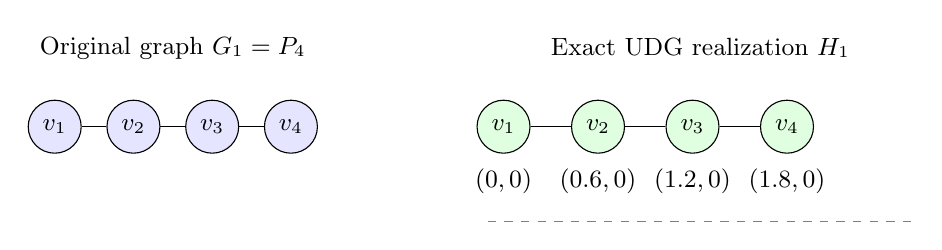
\begin{tikzpicture}[scale=1, every node/.style={font=\small}]
% Left: abstract graph
\node at (1.5,2.4) {Original graph $G_1=P_4$};
\node[circle,draw,fill=blue!10] (a1) at (0,1.4) {$v_1$};
\node[circle,draw,fill=blue!10] (a2) at (1,1.4) {$v_2$};
\node[circle,draw,fill=blue!10] (a3) at (2,1.4) {$v_3$};
\node[circle,draw,fill=blue!10] (a4) at (3,1.4) {$v_4$};
\draw (a1)--(a2)--(a3)--(a4);

% Right: realization
\node at (8.2,2.4) {Exact UDG realization $H_1$};
\draw[dashed,gray] (5.5,0.2) -- (10.9,0.2);
\node[circle,draw,fill=green!12] (b1) at (5.7,1.4) {$v_1$};
\node[circle,draw,fill=green!12] (b2) at (6.9,1.4) {$v_2$};
\node[circle,draw,fill=green!12] (b3) at (8.1,1.4) {$v_3$};
\node[circle,draw,fill=green!12] (b4) at (9.3,1.4) {$v_4$};
\draw (b1)--(b2)--(b3)--(b4);
\node[below=2pt of b1] {$(0,0)$};
\node[below=2pt of b2] {$(0.6,0)$};
\node[below=2pt of b3] {$(1.2,0)$};
\node[below=2pt of b4] {$(1.8,0)$};
\end{tikzpicture}
\end{center}

\subsection{Example 2: a property-preserving UDG for bipartite coloring}

Let
\[
G_2 = K_{3,3}.
\]
This graph is bipartite, hence
\[
\chi(G_2)=2.
\]
Instead of preserving exact structure, preserve the property
\[
P(G) := \text{``$G$ is $2$-colorable''}.
\]
Choose as UDG target the cycle
\[
H_2=C_6.
\]
Then $H_2$ is a UDG and
\[
\chi(H_2)=2.
\]
Thus we have a property-preserving example:
\[
H_2\in\UDG,
\qquad
\chi(G_2)\le 2 \iff \chi(H_2)\le 2,
\qquad
\chi(G_2)=\chi(H_2)=2.
\]

\begin{center}
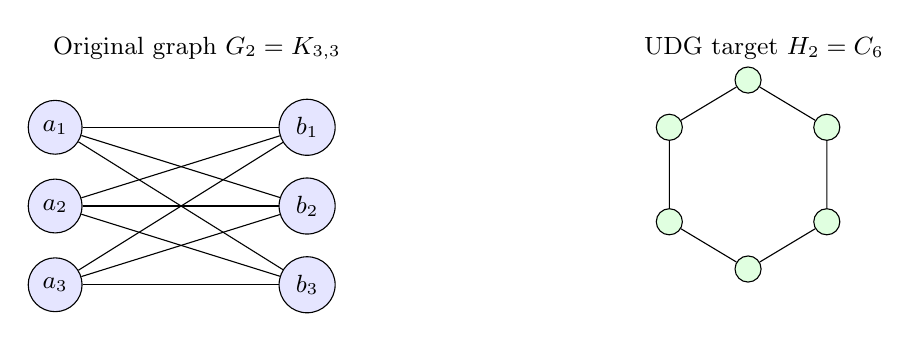
\begin{tikzpicture}[scale=1, every node/.style={font=\small}]
\node at (1.8,4.2) {Original graph $G_2=K_{3,3}$};
\foreach \i/\y in {1/3.2,2/2.2,3/1.2} {
  \node[circle,draw,fill=blue!10] (L\i) at (0,\y) {$a_\i$};
  \node[circle,draw,fill=blue!10] (R\i) at (3.2,\y) {$b_\i$};
}
\foreach \i in {1,2,3}{
  \foreach \j in {1,2,3}{
    \draw (L\i)--(R\j);
  }
}

\node at (9.0,4.2) {UDG target $H_2=C_6$};
\foreach \name/\x/\y in {c1/7.8/3.2,c2/8.8/3.8,c3/9.8/3.2,c4/9.8/2.0,c5/8.8/1.4,c6/7.8/2.0} {
  \node[circle,draw,fill=green!12] (\name) at (\x,\y) {};
}
\draw (c1)--(c2)--(c3)--(c4)--(c5)--(c6)--(c1);
\end{tikzpicture}
\end{center}

\subsection{Example 3: a property-preserving UDG for $3$-colorability}

Let $G_3$ be the Petersen graph. It is well known that
\[
\chi(G_3)=3.
\]
Take the UDG target
\[
H_3=C_5.
\]
Since an odd cycle has chromatic number $3$,
\[
\chi(H_3)=3.
\]
Therefore the chosen property
\[
P(G) := \text{``$G$ is $3$-colorable''}
\]
is preserved in the sense that
\[
H_3\in\UDG,
\qquad
\chi(G_3)\le 3 \iff \chi(H_3)\le 3,
\qquad
\chi(G_3)=\chi(H_3)=3.
\]

\begin{center}
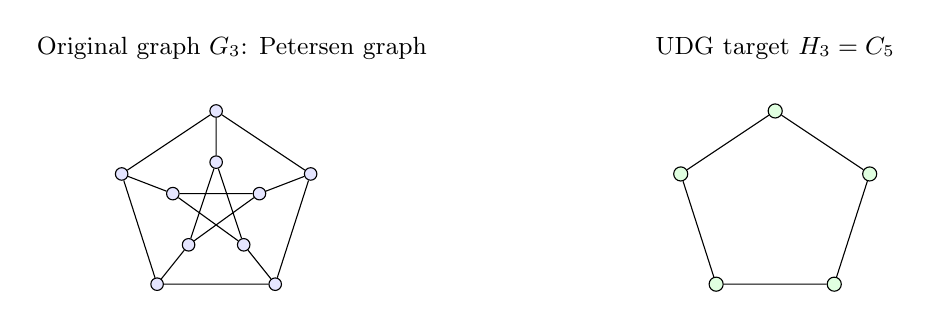
\begin{tikzpicture}[scale=1, every node/.style={font=\small}]
\node at (2.0,4.6) {Original graph $G_3$: Petersen graph};
% outer pentagon
\foreach \name/\x/\y in {o1/1.8/3.8,o2/3.0/3.0,o3/2.55/1.6,o4/1.05/1.6,o5/0.6/3.0} {
  \node[circle,draw,fill=blue!10,inner sep=1.6pt] (\name) at (\x,\y) {};
}
% inner star
\foreach \name/\x/\y in {i1/1.8/3.15,i2/2.35/2.75,i3/2.15/2.1,i4/1.45/2.1,i5/1.25/2.75} {
  \node[circle,draw,fill=blue!10,inner sep=1.6pt] (\name) at (\x,\y) {};
}
\draw (o1)--(o2)--(o3)--(o4)--(o5)--(o1);
\draw (i1)--(i3)--(i5)--(i2)--(i4)--(i1);
\draw (o1)--(i1) (o2)--(i2) (o3)--(i3) (o4)--(i4) (o5)--(i5);

\node at (8.9,4.6) {UDG target $H_3=C_5$};
\foreach \name/\x/\y in {p1/8.9/3.8,p2/10.1/3.0,p3/9.65/1.6,p4/8.15/1.6,p5/7.7/3.0} {
  \node[circle,draw,fill=green!12,inner sep=1.8pt] (\name) at (\x,\y) {};
}
\draw (p1)--(p2)--(p3)--(p4)--(p5)--(p1);
\end{tikzpicture}
\end{center}

\subsection{Example 4: a property-preserving UDG for chromatic number $4$}

Let $G_4=W_5$ denote the odd wheel obtained from a $5$-cycle by adding a hub adjacent to every cycle vertex. Then
\[
\chi(G_4)=4.
\]
Choose the UDG target
\[
H_4=K_4.
\]
The complete graph $K_4$ is a UDG, for example by placing four points sufficiently close together in the plane. Moreover,
\[
\chi(H_4)=4.
\]
Hence this illustrative property-preserving transform satisfies
\[
H_4\in\UDG,
\qquad
\chi(G_4)=\chi(H_4)=4,
\qquad
\chi(G_4)\le 4 \iff \chi(H_4)\le 4.
\]

\begin{center}
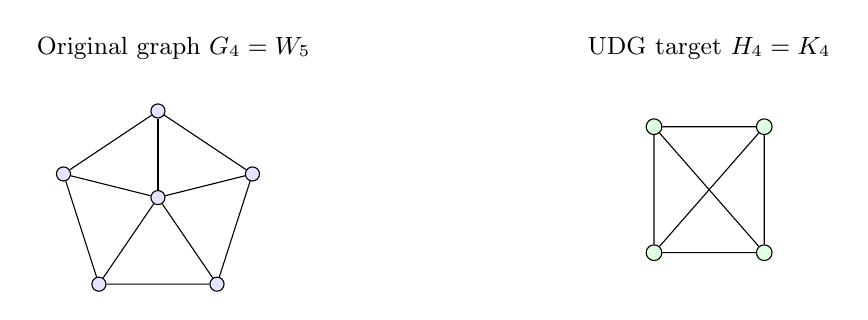
\begin{tikzpicture}[scale=1, every node/.style={font=\small}]
\node at (2.0,4.4) {Original graph $G_4=W_5$};
\foreach \name/\x/\y in {w1/1.8/3.6,w2/3.0/2.8,w3/2.55/1.4,w4/1.05/1.4,w5/0.6/2.8,wh/1.8/2.5} {
  \node[circle,draw,fill=blue!10,inner sep=1.8pt] (\name) at (\x,\y) {};
}
\draw (w1)--(w2)--(w3)--(w4)--(w5)--(w1);
\foreach \v in {w1,w2,w3,w4,w5}{\draw (wh)--(\v);} 

\node at (8.8,4.4) {UDG target $H_4=K_4$};
\foreach \name/\x/\y in {k1/8.1/3.4,k2/9.5/3.4,k3/8.1/1.8,k4/9.5/1.8} {
  \node[circle,draw,fill=green!12,inner sep=2pt] (\name) at (\x,\y) {};
}
\draw (k1)--(k2)--(k3)--(k4)--(k1)--(k3) (k2)--(k4);
\end{tikzpicture}
\end{center}

\subsection{Summary of the examples}

\begin{center}
\begin{tabular}{@{}llll@{}}
\toprule
Example & Original graph & UDG target & Preserved feature \\
\midrule
1 & $P_4$ & $P_4$ & exact graph structure / isomorphism \\
2 & $K_{3,3}$ & $C_6$ & bipartiteness, $2$-colorability, $\chi=2$ \\
3 & Petersen graph & $C_5$ & $3$-colorability, $\chi=3$ \\
4 & $W_5$ & $K_4$ & $4$-colorability, $\chi=4$ \\
\bottomrule
\end{tabular}
\end{center}

\newpage

\section{Conclusion and next steps}

The revised thesis direction is stronger than the original one because it no longer assumes that the input is already a unit-disk graph. Instead, it treats graph-to-UDG transformation, typed verification, and hardware lowering as first-class concerns. The paper has therefore shifted from a language for coloring on UDGs to a language for \emph{certified transformation into UDG-compatible instances} for graph coloring on neutral-atom hardware.

The paper has also integrated seven concrete, polynomial-time heuristics for property-preserving UDG transformation, each with full complexity analysis, formal safety guarantees, and typed integration into the language. The key insight is that exact embedding is NP-hard, but constructing a safe UDG \emph{supergraph} that preserves coloring properties is polynomial and well-structured.

The most immediate next steps are:
\begin{enumerate}[label=(\arabic*)]
    \item refine the minimal type system into a complete formal typing judgment,
    \item define certificate forms for exact realization and property preservation,
    \item implement the seven heuristics and conduct empirical evaluation on benchmark graph families,
    \item make the backend interface precise enough to model QuEra lowering,
    \item extend the examples into formal case studies and provide performance benchmarks,
    \item prove soundness results linking well-typed programs to well-defined transformed instances and decoded solutions.
\end{enumerate}

\end{document}